
\ifdefined\ishandout
\documentclass[11pt,english,handout]{beamer}
\else
\documentclass[11pt,english]{beamer}
\fi

%\documentclass[11pt]{beamer}
\usepackage{mathptmx}
\renewcommand{\sfdefault}{lmss}
\renewcommand{\familydefault}{\sfdefault}
\usepackage[T1]{fontenc}
\usepackage[latin9]{inputenc}
\usepackage{amsmath}
\usepackage{amssymb}
\usepackage{graphicx}
\PassOptionsToPackage{normalem}{ulem}
\usepackage{ulem}
\usepackage{caption}
\captionsetup{labelformat=empty}
\usepackage{bbm}
\usepackage{upgreek}
\usepackage{graphicx}
\setbeamertemplate{section in toc}[sections numbered]
\makeatletter
\usepackage{caption} 
\captionsetup[table]{skip=10pt}
%%%%%%%%%%%%%%%%%%%%%%%%%%%%%% Textclass specific LaTeX commands.
% this default might be overridden by plain title style
\newcommand\makebeamertitle{\frame{\maketitle}}%
% (ERT) argument for the TOC
\AtBeginDocument{%
	\let\origtableofcontents=\tableofcontents
	\def\tableofcontents{\@ifnextchar[{\origtableofcontents}{\gobbletableofcontents}}
	\def\gobbletableofcontents#1{\origtableofcontents}
}

%%%%%%%%%%%%%%%%%%%%%%%%%%%%%% User specified LaTeX commands.
%\documentclass[presentation]{beamer}


\def\Tiny{\fontsize{7pt}{8pt}\selectfont}
\def\Normal{\fontsize{8pt}{10pt}\selectfont}

\usetheme{Madrid}
\usecolortheme{lily}
%\setbeamercovered{transparent}
\useinnertheme{rounded}


\setbeamertemplate{footline}{\hfill\Normal{\insertframenumber/\inserttotalframenumber}}
%\setbeamertemplate{footline}{}

\setbeamertemplate{navigation symbols}{}

\newenvironment{changemargin}[2]{%
	\begin{list}{}{%
			\setlength{\topsep}{0pt}%
			\setlength{\leftmargin}{#1}%
			\setlength{\rightmargin}{#2}%
			\setlength{\listparindent}{\parindent}%
			\setlength{\itemindent}{\parindent}%
			\setlength{\parsep}{\parskip}% 
		}%
		\item[]}{\end{list}}

\setbeamertemplate{footline}{\hfill\insertframenumber/\inserttotalframenumber}
\setbeamertemplate{navigation symbols}{}

%\usepackage{times}  % fonts are up to you
\usepackage{graphicx}
%\usepackage{graphics}
\usepackage{epsfig}
\usepackage{bm}
\usepackage{epsf}
\usepackage{float}
\usepackage[final]{pdfpages}
\usepackage{multirow}
\usepackage{colortbl}
\usepackage{xkeyval}
%\usepackage{sgame}
%\usepackage{pst-node}
\usepackage{listings}
\usepackage{ifthen}
%\usepackage{hyperref}
\usepackage{tikz}

%\usepackage{times}  % fonts are up to you
%\usepackage{graphicx}
%\usepackage{graphics}
\usepackage{epsfig,bm,epsf,float}
\usepackage[final]{pdfpages}
\usepackage{xcolor,multirow,colortbl}
\usepackage{xkeyval}
\usepackage{verbatim}
%\usepackage{sgame}
%\usepackage{pst-node}
\usepackage{listings}
%\usepackage{handoutWithNotes}
%\pgfpagesuselayout{3 on 1 with notes}[letterpaper,border shrink=5mm]
%\pgfpagesuselayout{2 on 1 with notes landscape}[letterpaper,border shrink=5mm]
\usepackage{setspace}
\usepackage{ragged2e}

\setbeamersize{text margin left=1em,text margin right=1em} % CambridgeUS spacing if you use default instead


%\pdfmapfile{+sansmathaccent.map}

% Table formatting
\usepackage{booktabs}


% Decimal align
\usepackage{dcolumn}
\newcolumntype{d}[0]{D{.}{.}{5}}


\global\long\def\expec#1{\mathbb{E}\left[#1\right]}
\global\long\def\var#1{\mathrm{Var}\left[#1\right]}
\global\long\def\cov#1{\mathrm{Cov}\left[#1\right]}
\global\long\def\prob#1{\mathrm{Prob}\left[#1\right]}
\global\long\def\one{\mathbf{1}}
\global\long\def\diag{\operatorname{diag}}
\global\long\def\expe#1#2{\mathbb{E}_{#1}\left[#2\right]}
\DeclareMathOperator*{\plim}{\text{plim}}

%\usefonttheme[onlymath]{serif}

\usepackage{appendixnumberbeamer}
\renewcommand{\thefootnote}{}

\setbeamertemplate{footline}
{
	\leavevmode%
	%   \hbox{%
	%      \begin{beamercolorbox}[wd=\paperwidth,ht=2.25ex,dp=1ex,right]{date in head/foot}%
	%\usebeamerfont{date in head/foot}\insertshortdate{}\hspace*{2em}%
	\hfill
	%turning the next line into a comment, erases the frame numbers
	\insertframenumber{}\hspace*{2ex}\vspace{1ex}
	
	%    \end{beamercolorbox}}%
}

\definecolor{blue}{RGB}{0, 0, 210}
\definecolor{red}{RGB}{170, 0, 0}

\makeatother

\usepackage[english]{babel}

\usepackage{tikz}
\newcommand*\circled[1]{\tikz[baseline=(char.base)]{             \node[circle,ball color=structure.fg, shade,   color=white,inner sep=1.2pt] (char) {\tiny #1};}} 

\makeatletter
\let\save@measuring@true\measuring@true
\def\measuring@true{%
	\save@measuring@true
	\def\beamer@sortzero##1{\beamer@ifnextcharospec{\beamer@sortzeroread{##1}}{}}%
	\def\beamer@sortzeroread##1<##2>{}%
	\def\beamer@finalnospec{}%
}
\makeatother



\setbeamersize{text margin left= .8em,text margin right=1em} 
\newenvironment{wideitemize}{\itemize\addtolength{\itemsep}{10pt}}{\enditemize}
\newenvironment{wideitemizeshort}{\itemize}{\enditemize}

\newcommand{\indep}{\perp\!\!\!\!\perp} 

\begin{document}

%% Title slide
\begin{frame}[noframenumbering]{}
\vspace{0.5cm}
\title[]{Chapter 3: Asymptotic Statistics}
\author{Jonathan Roth}
\date{Mathematical Econometrics I \\ Brown University\\} 
\titlepage {\small{}\ }\thispagestyle{empty} \vspace{-30pt}

\end{frame}

 
\begin{frame}{Outline}

1. Overview
\vspace{0.8cm}

2. LLN, CLT, and CMT
\vspace{0.8cm}

3. Putting Asymptotics into Practice

\end{frame}


\begin{frame}{Motivation}

\begin{wideitemize}
	
\item 
We've seen how we can test hypotheses about population means using information from the sample mean $\hat\mu$ when it is \textbf{normally distributed} with a known variance

\item
This situation arises when we know that $Y_i\sim \mathrm{N}(\mu,\sigma^2)$ with known $\sigma$	

\item
But this situation is rare... how do we ``do inference'' more generally? 

\pause

\item
Fortunately, the assumption of normally distributed sample means turns out to be a good \textbf{approximation} when samples are large

\pause
\item
What we mean by a ``good approximation'' is formalized by asymptotic statistics,  which considers the distribution of $\hat\mu$ in the limit as $N \rightarrow \infty$
	
\end{wideitemize}		

\end{frame}


\begin{frame}{Overview of Important Results}
	
\begin{wideitemize}

\item The \textbf{Law of Large Numbers} (LLN) says that when $N$ is large, $\hat\mu$ is close to $\mu$ with very high probability

\pause
\item The \textbf{Central Limit Theorem} (CLT) says that when $N$ is large, the distribution of $\hat\mu$ is approximately normally distributed with mean $\mu$ and variance $\sigma^2/N$

\pause
\item The \textbf{Continuous Mapping Theorem} says that when $N$ is large, continuous functions of $\hat\mu$, say $g(\hat\mu)$, are also close to $g(\mu)$


\end{wideitemize}	
\end{frame}


\begin{frame}{Outline}

\textcolor{red!75!green!50!blue!25!gray}{1. Overview} $\checkmark$
\vspace{0.8cm}

2. LLN, CLT, and CMT
\vspace{0.8cm}

\textcolor{red!75!green!50!blue!25!gray}{3. Putting Asymptotics into Practice}

\end{frame}


\begin{frame}{Convergence in Probability}
	
\begin{wideitemize}
\item
Intuitively, a random variable $X_N$ \textbf{converges in probability} to $x$ if the probability that $X_N$ is ``close to'' $x$ is almost 1 when $N$ is large

\pause
\item
Formally, we say $X_N$ converges in probability to $x$,  $X_N \rightarrow_p x$ or $plim \, X_N =x $, if for all $\epsilon > 0$, 

$$P(|X_N - x| > \epsilon) \rightarrow 0 $$

\pause
\item 
If $X_N \rightarrow_p x$ for a constant $x$, we say $X_N$ is \textit{consistent} for $x$

\pause
\item
Typically $x$ is a constant, although we will sometimes also say $X_N \rightarrow X$ for $X$ a random variable (using the same definition as above)
	
\end{wideitemize}

\end{frame}


\begin{frame}{Convergence in Probability (Cont.)}
	
\begin{wideitemize}

\item Useful fact: if $E[ (X_N - x)^2 ] \rightarrow 0$, then $X_N \rightarrow_p x$

\pause

\item 
\textbf{Proof} (you won't be responsible for this): \\

By the law of iterated expectations, 
\begin{align*}
E[ (X_N - x)^2 ]=& P( |X_N - x| > \epsilon ) E[ (X_N - x)^2 | |X_N - x| > \epsilon ] + \\
& P( |X_N - x| \leq \epsilon ) E[ (X_N - x)^2 | |X_N - x| \leq \epsilon ]	 \\
\pause \geq &  P( |X_N - x| > \epsilon ) \epsilon^2 + 0 
\end{align*}
\pause
\noindent This implies that 
$$P( |X_N - x|  > \epsilon ) \leq E[ (X_N - x)^2  ] / \epsilon^2 \text{ (Chebychev's Inequality)  }$$
\pause 
Hence, $E[ (X_N - x)^2  ] \rightarrow 0$ implies $P( |X_N - x|  > \epsilon ) \rightarrow 0$

\end{wideitemize}	
\end{frame}


\begin{frame}{Law of Large Numbers}
	
\begin{wideitemize}
	
\item \textbf{Law of Large Numbers}. Suppose that $Y_1,...,Y_N$ are drawn $iid$ from a distribution with $Var(Y_i) = \sigma^2 < \infty$. Then $$\hat\mu_N = \frac{1}{N} \sum_{i=1}^{N} Y_i \rightarrow_p \mu = E[Y_i]$$

\item
In words: as the sample gets large, the sample mean will be close to the population mean with high probability.

\pause
\item
\textbf{Proof:} We saw last chapter that $E[\hat\mu_N] = \mu$ and $Var(\hat\mu_N) = \sigma^2 / N$.  \\

Thus, $$Var(\hat\mu_N) = E[ (\hat\mu_N - \mu )^2 ] = \sigma^2/N \rightarrow 0 $$ \\

Hence, $\hat\mu_N \rightarrow_p \mu$ by our ``useful fact''. 
\end{wideitemize}	
	
\end{frame}



\begin{frame}{Laws of Large Numbers Illustration}
	\vspace{0.2cm}
	Distribution and mean of $\frac{1}{N}\sum_i Z_i$ when $Z_i\sim \mathrm{U}(0,1)$, $\mathbf{N=1}$
	
	\begin{center}
		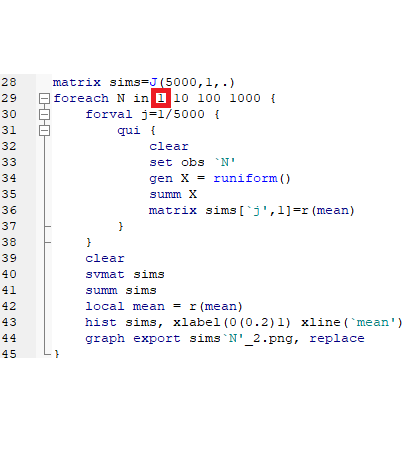
\includegraphics[scale=0.4]{Stata5.png} 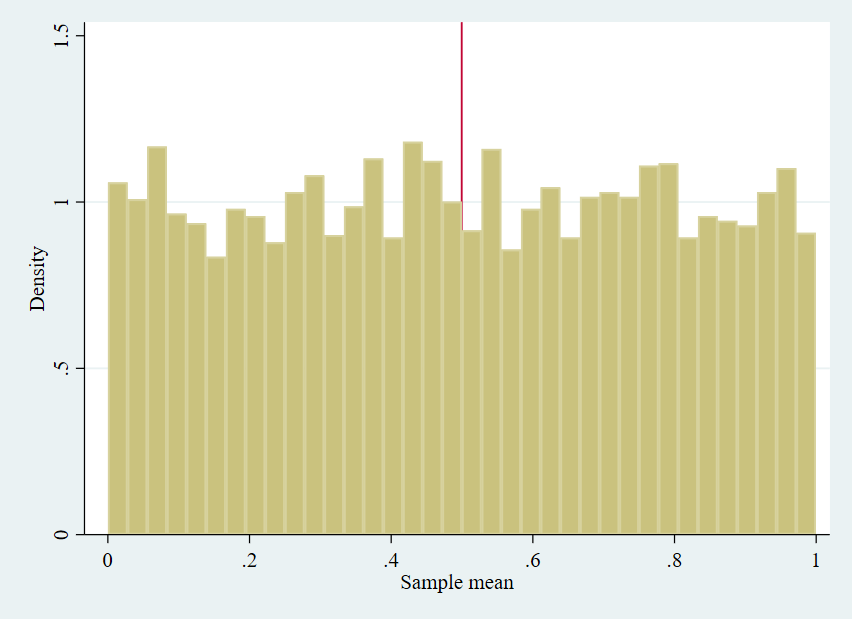
\includegraphics[scale=0.25]{sims1_2.png}
	\end{center}
	
\end{frame}

\begin{frame}{Laws of Large Numbers Illustration}
	\vspace{0.2cm}
	Distribution and mean of $\frac{1}{N}\sum_i Z_i$ when $Z_i\sim \mathrm{U}(0,1)$, $\mathbf{N=10}$
	
	\begin{center}
		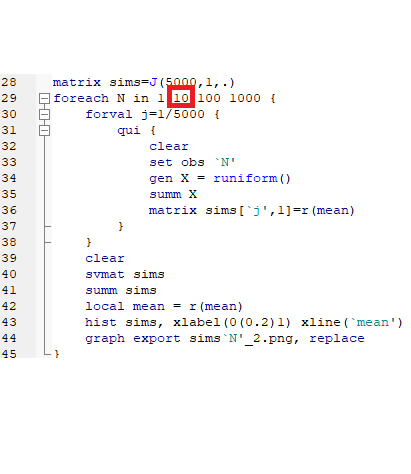
\includegraphics[scale=0.4]{Stata6.png} 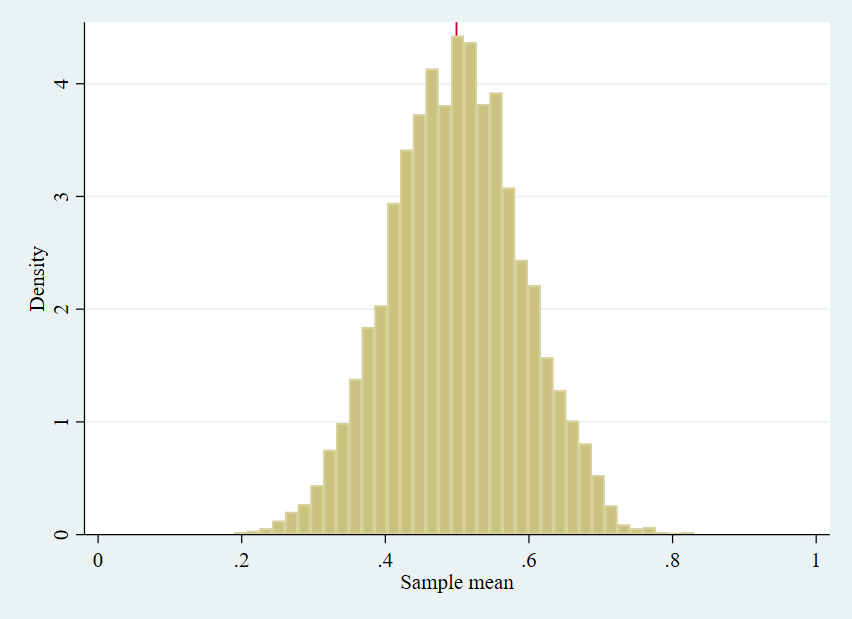
\includegraphics[scale=0.25]{sims10_2.png}
	\end{center}
	
\end{frame}

\begin{frame}{Laws of Large Numbers Illustration}
	\vspace{0.2cm}
	Distribution and mean of $\frac{1}{N}\sum_i Z_i$ when $Z_i\sim \mathrm{U}(0,1)$, $\mathbf{N=100}$
	
	\begin{center}
		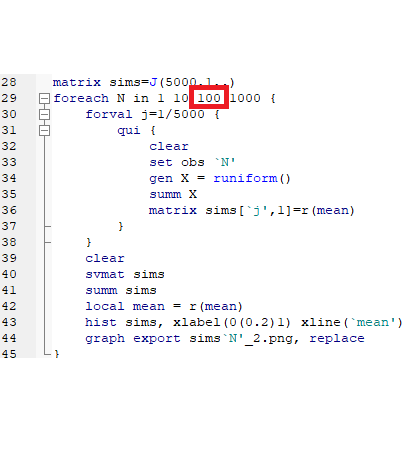
\includegraphics[scale=0.4]{Stata7.png} 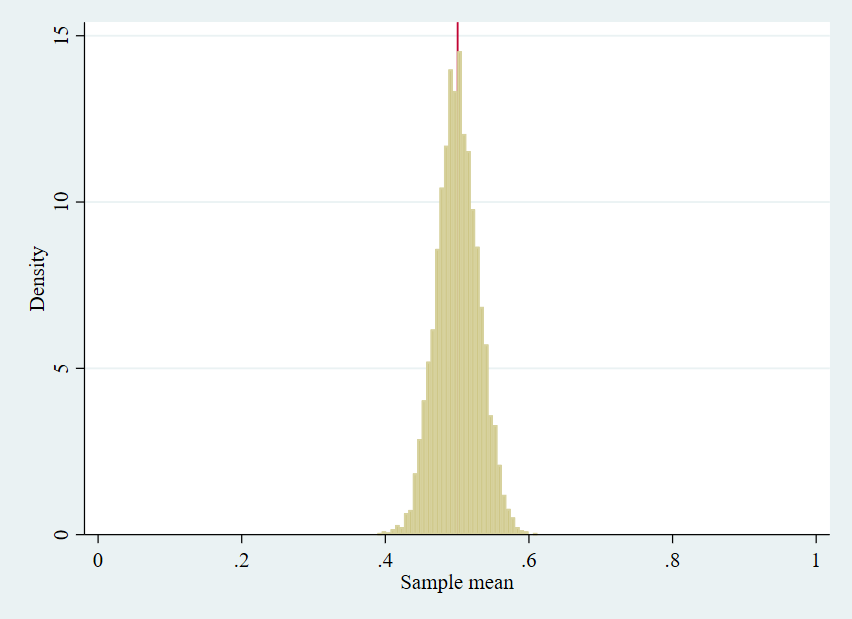
\includegraphics[scale=0.25]{sims100_2.png}
	\end{center}
	
\end{frame}

\begin{frame}{Laws of Large Numbers Illustration}
	\vspace{0.2cm}
	Distribution and mean of $\frac{1}{N}\sum_i Z_i$ when $Z_i\sim \mathrm{U}(0,1)$, $\mathbf{N=1000}$
	
	\begin{center}
		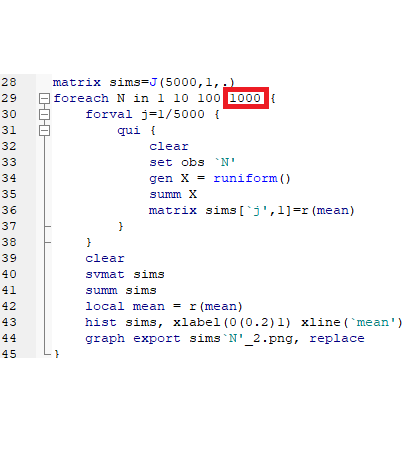
\includegraphics[scale=0.4]{Stata8.png} 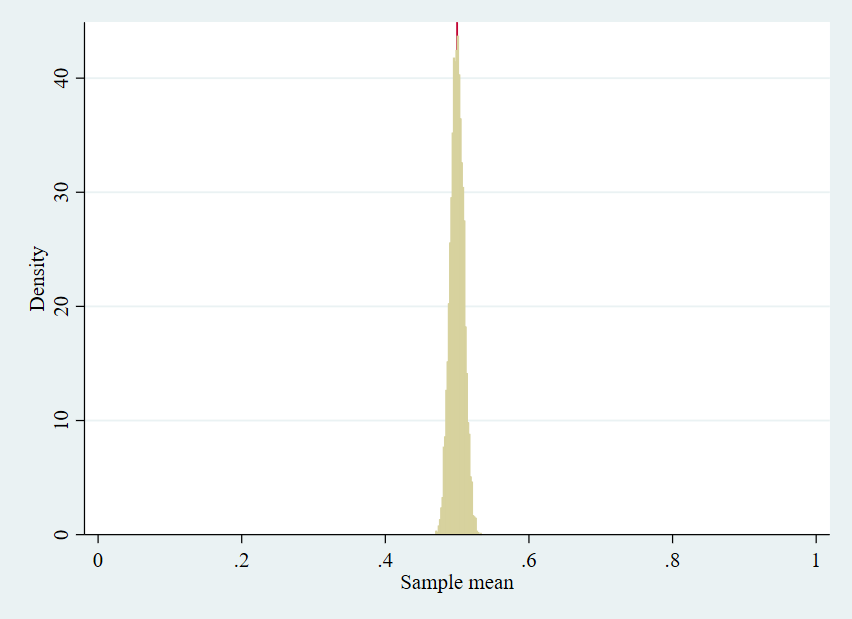
\includegraphics[scale=0.25]{sims1000_2.png}
	\end{center}
	
\end{frame}


\begin{frame}{Convergence in Distribution}
	
	\begin{wideitemize}

		\item
		You might have noticed that the distribution of $\hat\mu$ in the simulations looks close to a normal distribution as $N$ gets large
		
		\item
		The notion of \textbf{convergence in distribution} formalizes what it means for one distribution to be close to another distribution
		
		
		\pause
		\item
		Definition: We say that $X_N$ converges in distribution to a continuously distributed variable $X$, denoted $X_N \rightarrow_d X$ or $X_N \Rightarrow X$, if the CDF of $X_N$ converges (pointwise) to the CDF of $X$,
		
		$$F_{X_N}(x) \rightarrow F_{X}(x) \text{ for all } x$$ 
		
		
%		\pause
%		\item
%		\emph{Technical note}: if the limit $X$ is discrete, we only require $F_{X_N}(x) \rightarrow F_{X}(x)$ at points where $F(x)$ is continuous
%		
%			\begin{itemize}
%				\item
%				For example, if $X_N = 1/N$ and $X = 0$, then we say $X_N \rightarrow_d X$ even though $F_{X_N}(0) = 0$ for all $N$ while $F_X(0) = 1$
%			\end{itemize}
	\end{wideitemize}
	
\end{frame}


\begin{frame}{Central Limit Theorem}
\begin{wideitemize}

\item
\textbf{The Central Limit Theorem (CLT)} formalizes the sense in which sample means are approximately normally distributed in large samples

\pause
\item
Theorem: Suppose that $Y_1,...,Y_N$ are drawn $iid$ from a distribution with mean $\mu = E[Y_i]$ and variance $Var(Y_i) = \sigma^2 < \infty$. Then the sample mean $\hat\mu = \frac{1}{N} \sum_{i=1}^N Y_i$ satisfies

$$ \sqrt{N} (\hat\mu - \mu) \rightarrow_d N(0, \sigma^2) $$


\pause
\item
In words, the theorem says the following: 


\begin{enumerate}
\normalsize{
\item 
We can start with any distribution $Y_i$, possibly non-normal 

\item
If we take the average of the $Y_1,...,Y_N$ in a sample sufficiently large, the distribution of $\hat\mu = \frac{1}{N} \sum_i Y_i$ is (approximately) normal! 
}
\end{enumerate}

\end{wideitemize}	

\end{frame}



\begin{frame}{CLT Illustration}
	\vspace{0.2cm}
	Distributions of $\hat{\mu}=\frac{1}{N}\sum_i X_i$ vs. $\mathrm{N}(E[\hat\mu],Var(\hat{\mu}))$: $X_i\sim \mathrm{U}(0,1)$, $\mathbf{N=1}$
	
	\begin{center}
		
\includegraphics[scale=0.4]{Stata1.png} 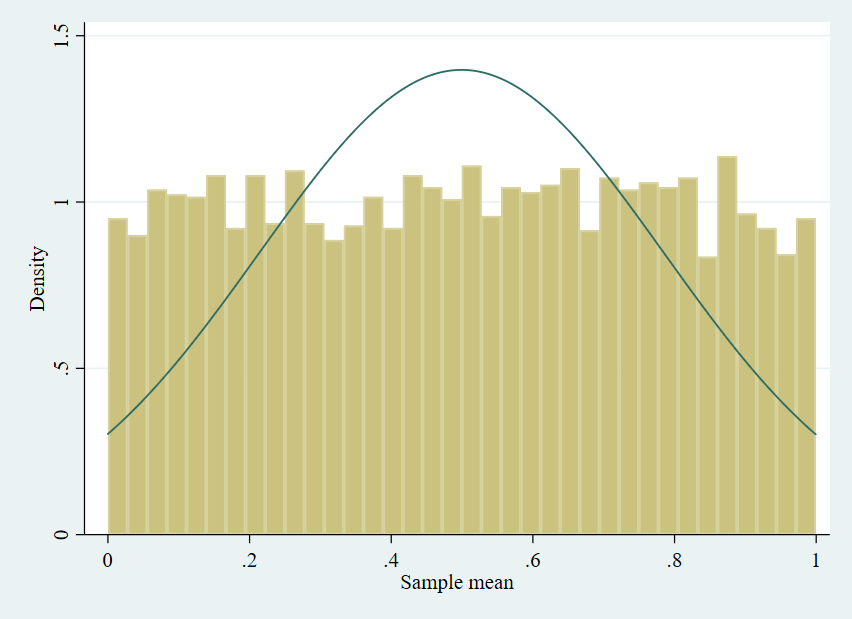
\includegraphics[scale=0.25]{sims1.png}
	\end{center}
	
\end{frame}

\begin{frame}{CLT Illustration}
	\vspace{0.2cm}
	Distributions of $\hat{\mu}=\frac{1}{N}\sum_i X_i$ vs. $\mathrm{N}(E[\hat\mu],Var(\hat{\mu}))$: $X_i\sim \mathrm{U}(0,1)$, $\mathbf{N=2}$
	
	\begin{center}
		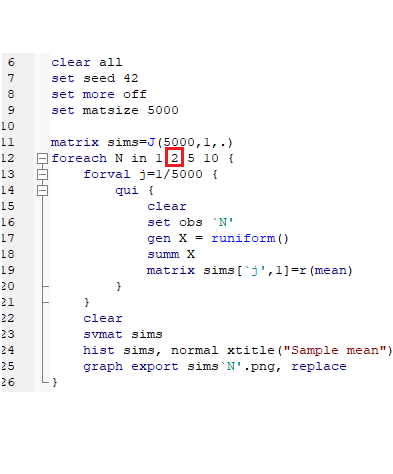
\includegraphics[scale=0.4]{Stata2.png} 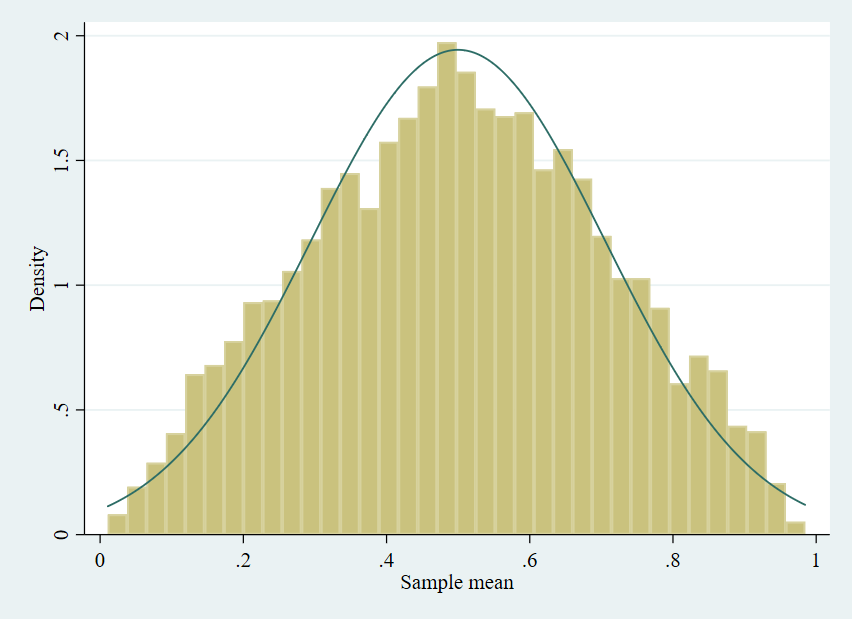
\includegraphics[scale=0.25]{sims2.png}
	\end{center}
	
\end{frame}

\begin{frame}{CLT Illustration}
	\vspace{0.2cm}
	Distributions of $\hat{\mu}=\frac{1}{N}\sum_i X_i$ vs. $\mathrm{N}(E[\hat\mu],Var(\hat{\mu}))$: $X_i\sim \mathrm{U}(0,1)$, $\mathbf{N=5}$
	
	\begin{center}
		
\includegraphics[scale=0.4]{Stata3.png} 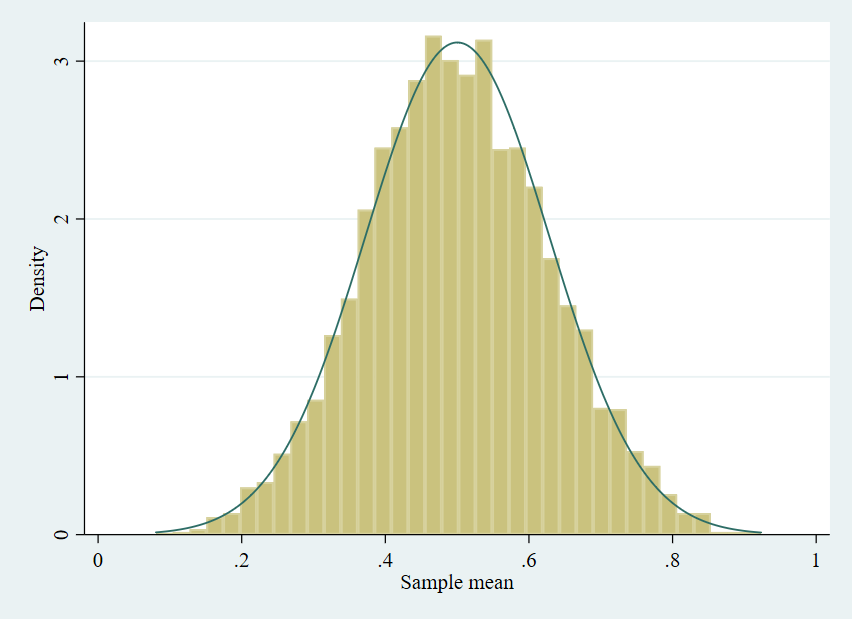
\includegraphics[scale=0.25]{sims5.png}
	\end{center}
	
\end{frame}

\begin{frame}{CLT Illustration}
	\vspace{0.2cm}
	Distributions of $\hat{\mu}=\frac{1}{N}\sum_i X_i$ vs. $\mathrm{N}(E[\hat\mu],Var(\hat{\mu}))$: $X_i\sim \mathrm{U}(0,1)$, $\mathbf{N=10}$
	
	\begin{center}
		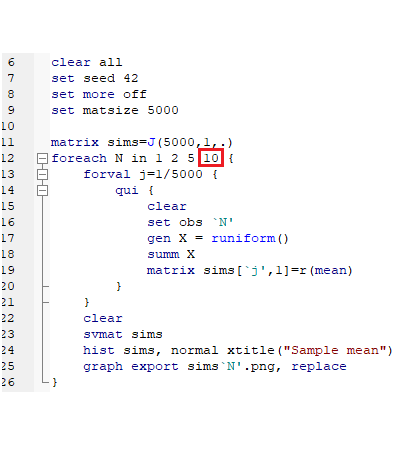
\includegraphics[scale=0.4]{Stata4.png} 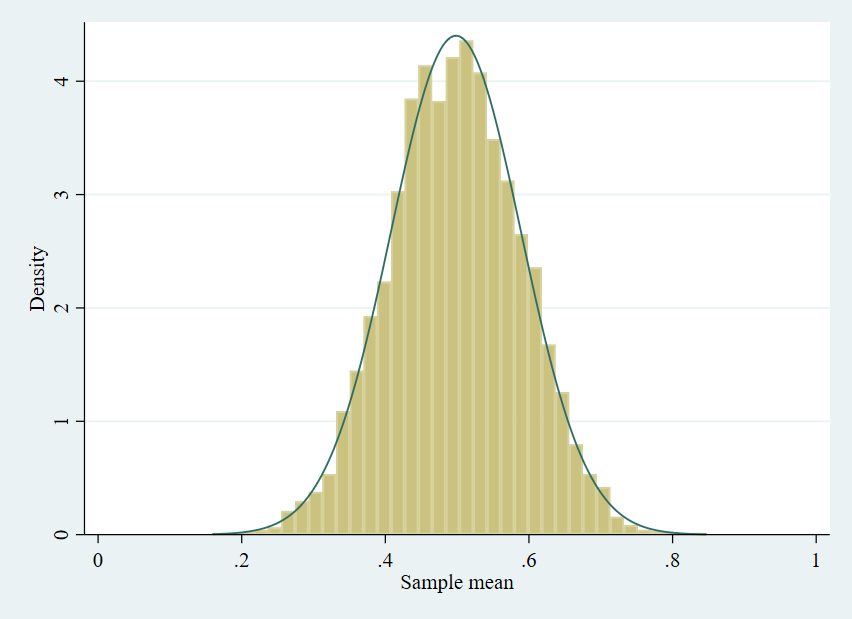
\includegraphics[scale=0.25]{sims10.png}
	\end{center}
	
\end{frame}


\begin{frame}{CLT Illustration II}
	\begin{center}
		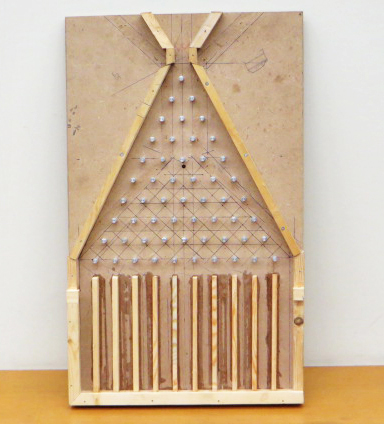
\includegraphics[width = 0.5\linewidth]{Galton_Board}
	\end{center}
	\href{https://www.youtube.com/watch?v=EvHiee7gs9Y}{https://www.youtube.com/watch?v=EvHiee7gs9Y}
\end{frame}


\begin{frame}
	\centering
	
\includegraphics[width = 0.5\linewidth]{mind-blown}
\end{frame}



\begin{frame}{Multivariate Versions}

\begin{wideitemize}
	\item 
	The results we've discussed extend naturally to the multivariate case
	
	\pause
	\item
	For a vector $\mathbf{X_N} \in \mathbb{R}^k$, we say $\mathbf{X_N} \rightarrow_p \mathbf{x}$ if each component of $\mathbf{X_N}$ converges in probability to each component of $\mathbf{x}$.
	
	\pause
	\item
	\textbf{LLN}: For $\hat{\boldsymbol{\mu}}_N$, the sample mean of $iid$ vectors $\mathbf{Y_1},...\mathbf{Y_N}$ with mean $\boldsymbol{\mu}$ and finite variance, $\hat{\boldsymbol{\mu}}_N \rightarrow_p \boldsymbol{\mu}$
	
	\pause
	\item
	For a vector $\mathbf{X_N} \in \mathbb{R}^k$, we say $\mathbf{X_N} \rightarrow_d \mathbf{X}$ for $\mathbf{X}$ continuously distributed if $F_{\mathbf{X_N}}(\mathbf{x}) \rightarrow F_{\mathbf{X}}(\mathbf{x})$ for all $\mathbf{x} \in \mathbb{R}^k$. 
	
	\item
	\textbf{CLT}: For $\hat{\boldsymbol{\mu}}_N$, the sample mean of $iid$ vectors $\mathbf{Y_1},...\mathbf{Y_N}$ with mean $\boldsymbol{\mu}$ and finite variance $\boldsymbol{\Sigma}$, $\sqrt{N} (\hat{\boldsymbol{\mu}}_N -\boldsymbol{\mu}) \rightarrow_d \mathrm{N}(\mathbf{0},\boldsymbol{\Sigma})$
	
	
\end{wideitemize}
	
\end{frame}


\begin{frame}{Continuous Mapping Theorem}

\begin{wideitemize}	

\item
Sometimes we are interested in functions of sample means (e.g., the $t$-statistic is a function of $\hat\mu$ and $\sigma$).

\pause
\item
The \textbf{continuous mapping theorem} (CMT) tells us about continuous functions of random variables that converge in distribution/probability

\pause
\item
Theorem: suppose $g(\cdot)$ is a continuous function\\
\vspace{.2cm}

If $X_N \rightarrow_p X$, then $g(X_N) \rightarrow_p g(X)$ \\
\vspace{.2cm}
\pause

If $X_N \rightarrow_d X$, then $g(X_N) \rightarrow_d g(X)$\\
\vspace{0.2cm}
\pause{}

Multivariate versions here too: If $\mathbf{X_N} \rightarrow_p \mathbf{X}$, then $g(\mathbf{X_N}) \rightarrow_p g(\mathbf{X})$ and if $\mathbf{X_N} \rightarrow_d \mathbf{X}$, then $g(\mathbf{X_N}) \rightarrow_d g(\mathbf{X})$

\end{wideitemize}

\end{frame}


\begin{frame}{Convergence of Sample Variance}
\begin{wideitemize}
\item
One useful application of the CMT is to show convergence in probability of the sample variance

\pause
\item
Let $\hat\sigma^2 = \frac{1}{N} \sum_{i=1}^N (Y_i - \hat\mu)^2$ be the sample variance of $Y_i$.

\pause
\item
Claim: if $Y_1,...,Y_N$ are $iid$ and $Var(Y_i^2)$ is finite, then $\hat\sigma^2 \rightarrow_p \sigma^2 = Var(Y_i)$. 

\pause
\item
Proof: \\

We can write the sample variance as $\hat\sigma^2 = \frac{1}{N} \sum_{i=1}^N Y_i^2 - \hat\mu^2$. \\ \vspace{.1cm} \pause

First term: by the LLN, $ \frac{1}{N} \sum_{i=1}^N Y_i^2 \rightarrow_p E[Y_i^2]$. \\ \vspace{.1cm} \pause

Second term: by the LLN, $\hat\mu \rightarrow_p \mu = E[Y_i]$. Thus, by the CMT, $\hat\mu^2 \rightarrow_p E[Y_i]^2$.\\ \vspace{.1cm} \pause

Thus, by the CMT again, $\frac{1}{N} \sum_{i=1}^N Y_i^2 - \hat\mu^2 \rightarrow_p E[Y_i^2] - E[Y_i]^2 = \sigma^2$. 

\end{wideitemize}		
\end{frame}

\begin{frame}{Slutsky's Lemma}

\begin{wideitemize}

\item
\textbf{Slutsky's lemma} (sometimes Slutsky's theorem) summarizes a few special cases of the CMT that are very useful. 

\pause
\item
Suppose that $X_N \rightarrow_p c$ for a constant $c$, and $Y_N \rightarrow_d Y$. Then: 

\item
$X_N + Y_N \rightarrow_d c + Y$. \pause

\item
$X_N Y_N \rightarrow_d c Y$. \pause

\item
If $c \neq 0$, then $Y_N/ X_N \rightarrow_d Y /c$. 

\pause
\item
Analogous versions apply for vector-valued random variables.
\end{wideitemize}
	
\end{frame}

\begin{frame}{Asymptotic Hypothesis Testing}

\begin{wideitemize}
\item
Recall that when $Y_i \sim \mathrm{N}(\mu,\sigma^2)$, we showed that the $t$-statistic $\hat{t} = \frac{\hat\mu - \mu_0}{\sigma / \sqrt{N}} \sim  \mathrm{N}(0,1)$ under $H_0: \mu = \mu_0$.

\pause
\item 
Thus, when $Y_i \sim \mathrm{N}(\mu,\sigma^2)$, we had that $Pr(|\hat t| > 1.96) = 0.05$ under the null.

\pause
\item
Now, suppose that $Y_i$ is not normally distributed and we don't know its variance.

\pause
\item
By CLT, $\sqrt{N} (\hat\mu - \mu_0) \rightarrow_d N(0,\sigma^2)$.\\
By CMT and LLN (as shown above), $\hat\sigma \rightarrow_p \sigma$. 

\pause
\item
Thus, by Slutsky's lemma, $\hat{t} = \dfrac{\hat\mu - \mu_0}{ \hat\sigma /\sqrt{N} } \rightarrow_d N(0,1)$.

\pause
\item
Hence, asymptotically $Pr( |\hat{t}| > 1.96 ) \rightarrow 0.05$, even though $Y_i$ is not normal and $\hat\sigma$ is estimated! We can hypothesis test just like before.

\end{wideitemize}	
	
\end{frame}


\begin{frame}{Asymptotic Confidence Intervals}

\begin{wideitemize}
\item
Similarly, when $Y_i$ was normal w/ $\sigma$ known, we showed the confidence interval $\hat\mu \pm 1.96 \sigma/\sqrt{N}$ contained the true $\mu$ 95\% of the time

\pause
\item
Analogously, when $Y_i$ is non-normal with unknown variance, $\hat\mu \pm 1.96 \hat\sigma/\sqrt{N}$ contains the true $\mu$ with probability approaching 95\% as $N$ grows large.

\end{wideitemize}
	
\end{frame}

\begin{frame}{Outline}

\textcolor{red!75!green!50!blue!25!gray}{1. Overview} $\checkmark$
\vspace{0.8cm}

\textcolor{red!75!green!50!blue!25!gray}{2. LLN, CLT, and CMT} $\checkmark$
\vspace{0.8cm}

3. Putting Asymptotics into Practice

\end{frame}

\begin{frame}{Example -- Oregon Health Insurance Experiment}
	
\begin{center}
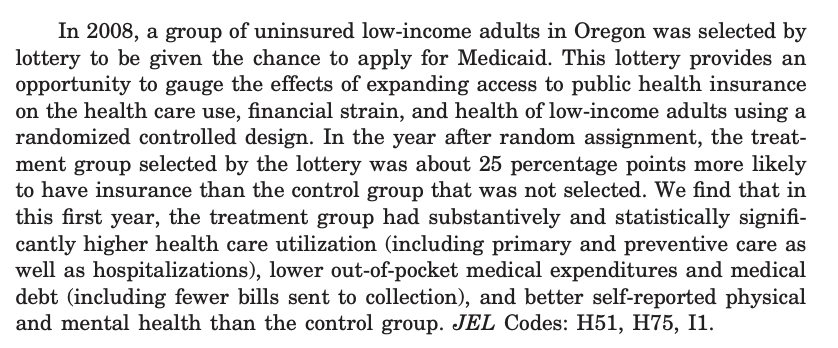
\includegraphics[width = 0.9 \linewidth]{ohie-abstract}	
\end{center}
\end{frame}


\begin{frame}{Sample Means for Depression Outcome}

\begin{tabular}{lll}
 & Control Group & Treated Group \\
 Mean & 0.329 & 0.306\\
 SD & 0.470 &  0.461 \\
 N & 10426 & 13315  
\end{tabular}

\pause
\begin{wideitemize}
	\item
	Say we want a CI for the population mean in the control group
	\pause
	\item
	We have $$\hat\mu \pm 1.96 \times \hat\sigma / \sqrt{N} = \pause{} 0.329 \pm 1.96 \times 0.470 / \sqrt{10426} =  \pause{} [0.319, 0.338] $$
	
	\pause
	\item
	What about for the treated group? 
	\pause
	$$\hat\mu \pm 1.96 \times  \hat\sigma / \sqrt{N} = \pause{} 0.306 \pm 1.96 \times 0.461 / \sqrt{13315} =  \pause{} [0.298, 0.313] $$
\end{wideitemize}

\end{frame}



\begin{frame}{CIs for Treatment Effects in Experiments}
	
	\begin{wideitemize}
		\item
		We showed previously that in an experiment, the average treatment effect is given by 
		
		$$\tau = E[Y_i(1) - Y_i(0)] = E[Y_i | D_i = 1] - E[Y_i | D_i = 0].$$
		
		i.e. the difference in population means between the treated and control groups.
		\pause
		\item
		How can we form confidence intervals (or test hypotheses) about the treatment effect? 
						
	\end{wideitemize}
	
\end{frame}

\begin{frame}{Mean and variance of the difference-in-means}
\begin{wideitemize}
			\item
			Let $\bar{Y}_1 = \frac{1}{N_1} \sum_{i: D_i = 1}  Y_i $ be the sample mean for the treated group. \\
			Let $\bar{Y}_0 = \frac{1}{N_0} \sum_{i: D_i = 0}  Y_i $ be the sample mean for the control group. 
			
			\pause 
			\item
			Since $\bar{Y}_1,\bar{Y}_0$ are each sample means, we have that \pause 
			\begin{align*}
			& E[\bar{Y}_1] = \mu_1, \hspace{2cm} Var(\bar{Y}_1) = \sigma_1^2 / N_1 \\
			& E[\bar{Y}_0] = \mu_0, \hspace{2cm} Var(\bar{Y_0}) = \sigma_0^2 / N_0 
			\end{align*} 
		\noindent where $\mu_d = E[Y_i \mid D_i=d]$ and $\sigma_d^2 = Var(Y_i \mid D_i = d)$.
		
		\
		
			\item
			Let $\hat\tau= \bar{Y}_1 - \bar{Y}_0$. It follows that $E[\hat\tau] = \pause{}\mu_1 - \mu_0 = \tau$ and
			\begin{align*}
			Var( \hat\tau ) &=  \pause{} \sigma_1^2 / N_1 +  \sigma_0^2 / N_0 + 2 Cov(\bar{Y_1}, \bar{Y_0})\\
			& = \pause{}\sigma_1^2 / N_1 +  \sigma_0^2 / N_0 
					\end{align*}
			\noindent where the fact that the samples are independent implies that $Cov(\bar{Y_1}, \bar{Y_0}) = 0$.
\end{wideitemize}
\end{frame}

\begin{frame}
	\begin{wideitemize}
		\item
		We just showed that in an experiment $$E[\hat\tau] = \tau \text{ and } Var(\hat\tau) = \sigma_1^2/N_1 + \sigma_0^2 / N_0$$ where $\hat\tau$ is the difference in sample means btwn the treated/control groups
		
		\item
		If we knew that $\hat\tau$ was normally distributed (and we knew $\sigma_1,\sigma_0$), then we could construct CIs of the form \pause
		$$ \hat\tau \pm 1.96 \sqrt{\sigma_1^2/N_1 + \sigma_0^2 / N_0} $$
		
		\pause 
		\item
		As with sample means, we do not know that $\hat\tau$ is normally distributed, but we can show that for $N$ large, it is \emph{approximately} normally distributed, which allows us to use CIs of the form
		
		 $$ \hat\tau \pm 1.96 \sqrt{\hat\sigma_1^2/N_1 + \hat\sigma_0^2 / N_0} ,$$
		 
		 for $\hat\sigma_d^2$ the estimated conditional variance.
	\end{wideitemize}
\end{frame}


%\pause\vspace{0.2cm}
%By the CLT,
%$$\left(   \begin{array}{c}\sqrt{N_1} \left( \bar{Y}_1 - E[Y_i(1)] \right)\\ 
%	\sqrt{N_0} \left( \bar{Y}_0 - E[Y_i(0)] \right) 
%\end{array}  \right) \rightarrow_d \mathrm{N}\left(\mathbf{0} , \left(\begin{array}{ll} Var(Y_i(1)) & 0 \\ 0 & Var(Y_i(0)) \end{array} \right) \right).$$



\begin{frame}{Showing Asymptotic Normality}

\begin{wideitemize}
\item
By the CLT, we have that $\sqrt{N_1} (\bar{Y_1} - \mu_1) \rightarrow_d \pause{} N(0,\sigma_1^2)$.  \pause
	
\item
Note that $\frac{N_1}{N} = \frac{1}{N} \sum_i D_i \rightarrow_p \pause{} E[D_i]$ by the LLN.

\pause
\item
Hence, applying the continuous mapping theorem,
\begin{align*}
\sqrt{N}(\bar{Y}_1 - E[Y_i(1)]) &= \pause{} (1/\sqrt{N_1/N}) \cdot \sqrt{N_1} (\bar{Y}_1 - E[Y_i(1)])\\ 
&\rightarrow_d (1/\sqrt{E[D_i]}) \cdot \mathrm{N}(0,Var(Y_i(1))) \\
& = \mathrm{N}\left(0, \frac{1}{E[D_i]} Var(Y_i(1)) \right)
\end{align*}

\pause
\item
Applying similar steps for $\bar{Y}_0$, we obtain that \pause
	$$\small \sqrt{N} \left(   \begin{array}{c}  \bar{Y}_1 - E[Y_i(1)] \\ 
	  \bar{Y}_0 - E[Y_i(0)] 
\end{array}  \right) \rightarrow_d \pause{} \mathrm{N}\left(0 , \left(\begin{array}{ll} \frac{1}{E[D_i]} Var(Y_i(1)) & 0 \\ 0 & \frac{1}{1-E[D_i]} Var(Y_i(0)) \end{array} \right) \right).$$

\end{wideitemize}
\end{frame}

\begin{frame}{Hypothesis Testing for Experiments (continued)}
\begin{wideitemize}
	\item
	We just showed that 
		$$\small \sqrt{N} \left(   \begin{array}{c}  \bar{Y}_1 - E[Y_i(1)] \\ 
		\bar{Y}_0 - E[Y_i(0)] 
	\end{array}  \right) \rightarrow_d \mathrm{N}\left(0 , \left(\begin{array}{ll} \frac{1}{E[D_i]} Var(Y_i(1)) & 0 \\ 0 & \frac{1}{1-E[D_i]} Var(Y_i(0)) \end{array} \right) \right).$$

\pause
\item
Applying the CMT, 
$$\sqrt{N} (\bar{Y}_1 -  \bar{Y_0} - E[Y_i(1) - Y_i(0)]) \rightarrow_d N(0 , \sigma^2),$$ 

\noindent where $\sigma^2 = \frac{1}{E[D_i]} Var(Y_i(1)) + \frac{1}{E[1-D_i]} Var(Y_i(0)) $ 

\pause

\item
We can thus form a 95\% confidence interval for $\tau = E[Y_i(1) - Y_i(0)]$,

$$\bar{Y}_1 - \bar{Y}_0 \pm  1.96 \hat\sigma / \sqrt{N},$$

\noindent where $\hat{\sigma}^2 = \frac{N}{N_1} \hat\sigma_1^2 + \frac{N}{N_0} \hat\sigma_0^2$, where $\hat{\sigma}^2_d$ is the sample variance for treatment group $d\in\{0,1\}$
\end{wideitemize}	
\end{frame}




\begin{frame}{Sample Means for Depression Outcome (Again)}
	
	\begin{tabular}{lll}
		& Control Group & Treated Group \\
		Mean & 0.329 & 0.306\\
		SD & 0.470 &  0.461 \\
		N & 10426 & 13315  
	\end{tabular}
	
	\pause
	\begin{wideitemize}
		\item
		Our point estimate of the treatment effect is $\hat\tau = \pause{} 0.306 - 0.329 = -0.023$.
		
		\pause
		\item
		Our CI for the treatment effect is: 
		\pause
		\begin{align*}
		&\hat\tau \pm 1.96 \times \sqrt{  \frac{1}{N_1}  \hat\sigma_1^2 + \frac{1}{N_0}  \hat\sigma_0^2  } = \pause{} \\ &-0.023 \pm 1.96 \times \sqrt{ \frac{1}{13315} 0.461^2 +  \frac{1}{10426} 0.470^2 } \\ &=  \pause{} [-0.035, -0.001] 
		\end{align*}
		
	\end{wideitemize}
	
\end{frame}




\begin{frame}{Hypothesis Testing under Unconfoundedness}
\begin{wideitemize}
\item
Recall that under unconfoundedness, $D_i \indep (Y_i(1),Y_i(0)) | X_i$, we have
$$ \underbrace{E[Y_i(1) - Y_i(0) | X_i =x]}_{CATE(x)} = E[Y_i | D_i = 1, X_i =x ] - E[Y_i | D_i = 0, X_i =x]$$ 

\noindent That is, within each value of $X_i$, it's as if we have an experiment. 

\pause
\item
By the same logic as for experiments, we have that 

$$\sqrt{N_x} (\bar{Y}_{1,x} -  \bar{Y}_{0,x} - E[Y_i(1) - Y_i(0) | X_i = x]) \rightarrow_d N(0 , \sigma_x^2),$$ 

\noindent where $N_x = |i : X_i = x|$ and 
$\sigma_x^2 = \frac{1}{E[D_i|X_i = x]} Var(Y_i(1) | X_i = x) + \frac{1}{E[1-D_i|X_i=x]} Var(Y_i(0)|X_i =x) $. 

\pause 
\item
So we can also do hyptothesis testing on $CATE(x)$ when $N_x$ is large.

\pause
\item
By averaging $CATE(x)$, we can do hypothesis testing / form CIs for $ATE$. 

\end{wideitemize}	
	
\end{frame}

\begin{frame}{The Challenge of Continuous $x$}
	
\begin{wideitemize} 
\item
We've shown thus far how we can estimate $CATE(x)$ when the number of observations with $X_i=x$ is large. 

\item
This works great when $X_i$ is binary (e.g. an indicator for college) or takes on a small number of discrete values (e.g. 50 states).

\pause
\item
But what about when $X_i$ is continuous? 

\pause
\item
For example, if $X_i$ is income, then to estimate $CATE(50,351)$, the theory we have says we need a large number of treated and control units both with income \$50,351. In most datasets, we won't have very many people with exactly this income.

\pause
\item
We thus need a different way of estimating conditional means when $X_i$ is continuously distributed.

\pause
\item
The next part of the course will focus on achieving this task using linear regression as an approximation to the CEF. 
\end{wideitemize}	
	
\end{frame} 

\end{document}
}
